\documentclass{beamer}
\usetheme{afm}

\title{Arbitrage-Free Pricing Theory}
\subtitle{Let's refresh some useful concept}
\course{Advanced Financial Modelling}
\author{\href{mailto:matteo.sani@unisi.it}{Matteo Sani}}

\begin{document}
	\begin{frame}[plain]
		\maketitle
	\end{frame}        

\begin{frame}{}
\begin{block}{Disclaimer}	
Concerning this part I am assuming that:
\begin{itemize}
\item you know what is a random process;
\item you know what is a stochastic differential equation (SDE);
\item you know a bit of stochastic calculus (Ito's lemma, Ito's integral\ldots);
\item you know (or have heard of) no-arbitrage pricing theorems;
\item you know (or have heard of) Monte Carlo Simulation.
\end{itemize}
\end{block}
\end{frame}	

\begin{frame}{Few Definitions}
		It may be helpful to explain (and recall) some of the more technical terms we are going to use.\newline
		
		\textbf{Sample space}: all possible future states or outcomes ($\Omega$) of a random process.\newline
		
		\textbf{(Probability) Measure} ($\mathbb{P}, \mathbb{Q}\ldots$): is a mapping which associates a probability to each element in the sample space. Two measures are \textbf{equivalent} if they agree "on what is possible". Note the word \emph{possible}: the two measures can have different probabilities for the same event, but must have the same \emph{null-set} $\{x\in {\mathbb{P}}\mid p (x)=0\}$. 
	\end{frame}

\begin{frame}{Few Definitions}
		\textbf{Contingent claim}: is a contract whose future payoff depends on the value of another “underlying” asset, or more generally, that is dependent on the realization of some uncertain future event $(S, X\ldots)$
		
		\begin{columns}
			\column{0.58\textwidth}
			\textbf{Filtrations}: are totally ordered collections of subsets that are used to model the information that is available at a given point in time ($\mathcal{F}_t$). 
			\column{0.35\textwidth}
				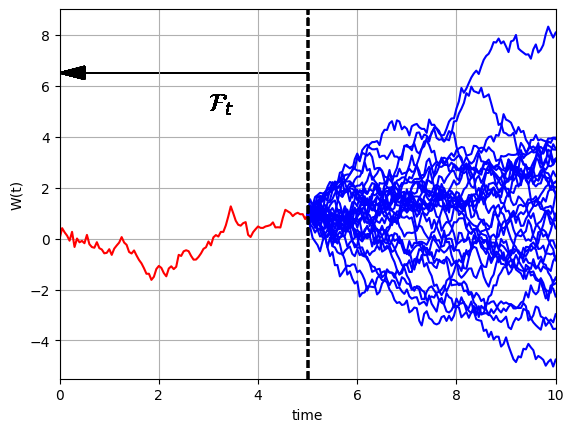
\includegraphics[width=0.8\linewidth]{filtration}
		\end{columns}
		
		\textbf{Martingale}: formally, a stochastic process is a martingale if
\begin{equation*} 
\mathbb{E}[X_{t+1}|\mathcal{F}_t] = X_t
\end{equation*}
or the conditional expectation of the next value in the sequence is equal to the present value, regardless of all prior values. 
It can be imagined as a \emph{drift-less} process
		\begin{equation*}
			dX = \cancel{\mu dt} + \sigma dW
		\end{equation*}
	\end{frame}

	\begin{frame}{Risk Neutral Pricing Foundations}
	Harrison and Pliska proved and formalized the following results:
	\begin{itemize}
		\item \textbf{The market is free of arbitrage if (and only if) there exists an \textcolor{red}{equivalent martingale measure} (EMM) (i.e. a risk-neutral measure).}
	\end{itemize}
	\vfill
	\end{frame}

\begin{frame}{Risk Neutral Pricing Foundations}
	\begin{itemize}
		\item Arbitrage opportunities rarely exist in practice. If and when they do, gains are extremely small, and are typically short-lived and difficult to spot. \textcolor{red}{Arbitrage exclusion in the mathematical model is close enough to reality}.
		\item An \textcolor{red}{equivalent martingale measure} $\mathbb{Q}$ is a probability measure on the space $\Omega$ such that
		\begin{enumerate}
			\item $\mathbb{Q}$ is equivalent to $\mathbb{P}$ (real world measure);
			\item for any asset $A$ and for each time $t$, $0\le t\le T$ there exists a price $\pi_t$
			\begin{equation*}
				\pi_t = \expect{Q}[D(t,T)V_A|\mathcal{F}_t]
			\end{equation*}
			which is a $\mathbb{Q}$-martingale.
		\end{enumerate}
	\end{itemize}
\end{frame}

\begin{frame}{Risk-Neutral Measure}
\begin{itemize}
\item  The difference between real-world and risk-neutral measures is in the treatment of the market price of risk.
\item If you tried to estimate the anticipated value of a stock based on how likely it is to go up or down, considering unique factors or market conditions that influence that specific asset, you would be including risk into the equation and, thus, would be looking at \textcolor{red}{real or physical probability}.
\item The \textcolor{red}{risk-neutral measure}, instead, allows determination of a market-consistent value without making any assumption about the market price of risk. That is useful because the price of risk is not directly observable, but the market prices used to calibrate a risk-neutral generator are.
\item The risk-neutral measure is a direct consequence of no arbitrage assumption. It is an \emph{implied probability distribution} from observable prices of tradable instruments, and used to determine \textcolor{red}{objective fair prices} for a financial instrument.
\end{itemize}
\end{frame}

\begin{frame}{Risk Neutral Pricing Foundations}
	Harrison and Pliska proved and formalized the following results:
	\begin{itemize}
		\item The market is free of arbitrage if (and only if) there exists an \textcolor{red}{equivalent martingale measure} (EMM) (i.e. a risk-neutral measure).
		\item \textbf{The market is complete if and only if the martingale measure is unique.}
		
		(Note that market completeness means that any contingent claim can be replicated by a portfolio, or in other words that every asset in every possible state of the world has a price.)
	\end{itemize}
	\vfill
\end{frame}

%\begin{frame}{Summary of Basic Definitions}
%	\begin{itemize}
%		\item The market is complete if and only if the martingale measure is unique.
%		\item In a complete and arbitrage-free market the price of any derivative is uniquely given, either by the value of the associated replicating strategy, or by the expectation of the discounted payoff under the risk-neutral measure
%		\begin{equation}
%			\Pi_t = \mathbb{E}^{\mathcal{Q}^0}[D(t,T)V_A|\mathcal{F}_t]
%			\label{eq:risk_neutral_pricing}
%		\end{equation}
%	\end{itemize}
%\end{frame}



%\begin{frame}{Martingale}
%	\begin{block}{Definition}
%		A \textcolor{red}{$\mathcal{F}_t$-martingale} is a (integrable and adapted) stochastic process which models a fair game with the following remarkable feature
%		\begin{equation}
%			\mathbb{E}[X_t|\mathcal{F}_s] = X_s
%		\end{equation}
%		so the best prediction for the future value $X_t$, given the knowledge $\mathcal{F}_s$ at time $s$ is the value at time $s$ itself, $X_s$.
%	\end{block}
%	%	\begin{block}{Properties}
%		\begin{itemize}
%			\item If $X_t$ is a stochastic process with diffusion coefficient $\sigma_t$, such that %which satisfies $\mathbb{E}\left[\left(\int_0^T\sigma^2_s ds\right)^{\frac{1}{2}}\right]<\infty$, and SDE 
%			$dX_t=\mu_t dt+\sigma_t dW_t$, then 
%			\begin{equation*}
%				X\text{ is a martingale } \iff X\text{ is drift-less } (\mu_t=0)
%			\end{equation*}
%		\end{itemize}	
%	\end{frame}

%\begin{frame}{Equivalent Martingale Measure}
%	\begin{block}{Definition}
%		An \textcolor{red}{equivalent martingale measure} $\mathbb{Q}$ is a probability measure on the space $\Omega$ such that
%		\begin{enumerate}
%			\item $\mathbb{Q}$ is equivalent to $\mathbb{P}$;
%			\item for any asset $A$ and for each time $t$, $0\le t\le T$ there exists a price $\pi_t$
%			\begin{equation*}
%				\pi_t = \expect{Q^0}[D(t,T)V_A|\mathcal{F}_t]
%			\end{equation*}
%			\item the "discounted asset price" is a $\mathbb{Q}$-martingale
%			\begin{equation*}
%				\pi_u = \expect{Q^0}[D(0,t)V_A(t)|\mathcal{F}_u], \quad\text{with }(t>u)
%			\end{equation*}
%		\end{enumerate}
%	\end{block}
%\end{frame}


\begin{frame}{Risk Neutral Pricing Foundations}
	Harrison and Pliska proved and formalized the following results:
	\begin{itemize}
		\item The market is free of arbitrage if (and only if) there exists an \textcolor{red}{equivalent martingale measure} (EMM) (i.e. a risk-neutral measure).
		\item The market is complete if and only if the martingale measure is unique;
		\item \textbf{In a complete and arbitrage-free market the price of any derivative is uniquely given, either by the value of the associated replicating strategy, or by the expectation of the discounted payoff under the risk-neutral measure}
		\begin{equation}
			\Pi_t = \expect{Q}[D(t,T)V_A|\mathcal{F}_t]
			\label{eq:risk_neutral_pricing}
		\end{equation}
	\end{itemize}
\end{frame}

\begin{frame}{What is the Monte Carlo Technique ?}
\begin{itemize}
	\item Our main goal is to compute prices with \cref{eq:risk_neutral_pricing}, which is not always analitycally solvable.
	\item Also many stochastic factors (stock prices, interest rates\ldots), influences the result, making predictions challenging. 
	\item \textbf{The Monte Carlo simulation technique} is the right tool to tackle this problems.
	\item It is a probability-based simulation method which exploits random sampling to analyse uncertain outcomes.
	\item Instead of relying on single-point estimates, \emph{it generates multiple scenarios based on probability distributions}. 
	\item This allows to assess the range of potential outcomes, not only a single average, providing a more comprehensive understanding of the problem in hand.
\end{itemize}
\end{frame}

\begin{frame}{How Does it Work ?}
\begin{enumerate}
	\item Identify the uncertain variables (e.g. stock prices, default probabilities\ldots);
	\item assign probability distributions to each, reflecting their potential movements;
	\item randomly sample from these distributions to simulate different scenarios;
	\item repeat this process hundreds, (or even thousands) of times: you will get a diverse landscape of potential outcomes, ready for analysis.
\end{enumerate}
\vspace{0.25cm}
\begin{columns}
	\column{0.4\linewidth}
	\hfill
	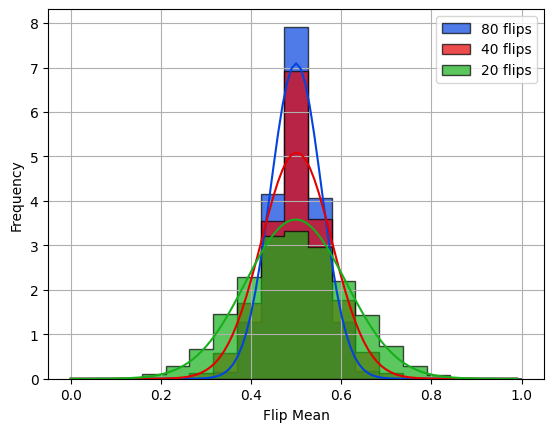
\includegraphics[width=0.8\linewidth]{central_limit_theorem}
	\vspace{0.7cm}
	\column{0.6\linewidth}
	The \textbf{Central Limit Theorem}: \emph{the sampling distribution of the mean is normally distributed, as long as the sample size is large enough}.
	
	\begin{enumerate}
		\item the best estimate of a quantity given by MC experiments is the \textbf{mean} of the simulation results;
		\item with a larger sample size, your sample mean is \textbf{more likely to be close to the real population mean} (more precise estimate).
	\end{enumerate}
\end{columns}
\begin{tikzpicture}[remember picture,overlay]
\node[xshift=-4.cm,yshift=-4.cm] (image) at (current page.center) {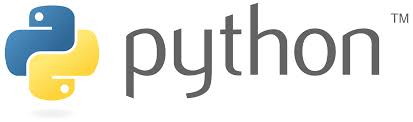
\includegraphics[width=80px]{python}};
\end{tikzpicture}
\end{frame}

\begin{homework}
\begin{frame}{\textcolor{white}{Homework}}
\begin{itemize}
\item[white]  You have determined the value of an interest rate derivative with a Monte Carlo simulation involving 50 scenarios which results in a contract value of 1.2 M€ $\pm$ 5\%. Unfortunately your boss ask you to determine more precisely the derivative value. If you have to meet him in 1 hour and each simulation lasts about 2.5 sec., what is the highest precision you can achieve ?
\item[white] Consider the process $Y(t) = 2^{W(t)}$, where $\{W(T):t\geq 0\}$ is a standard Brownian motion. Is this a martingale ?
\item[white]  Show that the exponential SDE
\begin{equation*}
dX_t = A_t X_tdW_t,\quad X_0=x_0
\end{equation*}
has the following solution
\begin{equation*}
X_t = x_0 e^{-\frac{1}{2}\int_0^t A_0^2 ds+\int_0^t A_s dB_s}
\end{equation*}
\end{itemize}
\textcolor{white}{Exercises for this part involves: SDE solving, martingale definition, Ito's lemma, and a bit of Monte Carlo theory.}
\end{frame}
\end{homework}

\end{document}
